\documentclass[12pt,a4paper,twocolumn]{article}
\usepackage[utf8]{inputenc}
\usepackage{amsmath}
\usepackage{amsfonts}
\usepackage{caption}
\usepackage{amssymb}
\usepackage{todonotes}
\usepackage{lipsum}
\author{Salvatore Prioli}
\title{\textbf{Assignment 1 - MM837}}
\begin{document}
\maketitle
\begin{abstract}
The aim of this report is to study the Fermi-Pasta-Ulam-Tsingu problem. 
After the end of the war, Enrico Fermi became interested in solving physical problems using computer machine.
In particular, these machine could be very useful when problems are not analitically solvable. 
The physical model studied is a long chain of particles coupled by spring. 
Fermi and his colleagues wanted to confirm the hypotesis that after some time the energy of the initial vibration would slowly be shared on all the other possible vibration of the system as stated by the equipartition theorem. 
However, results in disagreement with the equipartition thoeorem have been observed.
\end{abstract}
\section{Introduction}
The problem consist on some particles held together by some springs. All the particles can move up and down and the the first and the last one are connected to the wall (or ghost particles). The total number of degrees of freedom is $N$ where $N$ is the total number of particles. Every particle interacts with its closest right and left neighbor with a potential like the following:
\begin{equation}
	V(q)=\frac{1}{2}kx^2+\frac{1}{3}\alpha x^3 +\frac{1}{4}\beta x^4
\end{equation}
\section{Results}
\subsection{Hamilton's equations and force}
\todo[inline]{Riportare equazioni hamiltoniane del moto e espressioni per la forza}
The Hamiltonian of the system is the sum of the Kinetic and Potential energy:
\begin{equation}
\begin{split}
	H=&K+V\\
	K=&\frac{1}{2}\sum_{i=1}^N p_i^2\\
	V=&\sum_{\langle i,j \rangle}^N V(x_i-x_j)\\
%	V(x_i-x_{i+i})=&\frac{1}{2}(x_i-x_{i+1})^2\\
%	+&\frac{1}{3}(x_i-x_{i+1})^3\\
%	+&\frac{1}{4}(x_i-x_{i+1})^4\\
\end{split}
\end{equation}
%\begin{gather}
%	H=E=\sum_{i=1}^{N}\frac{1}{2}p_i^2+\sum_{\langle i,j \rangle} V(x_i-x_j)\\
%	V(x_i-x_{i+1})=\frac{1}{2}(x_i-x_{i+1})^2+\frac{1}{3}(x_i-x_{i+1})^3+\frac{1}{4}(x_i-x_{i+1})^4
%\end{gather}
The term in the potential energy is over adjacent pair of masses. Each pair of masses is counted only once. The complete form of the potential is:
\begin{equation}
\begin{split}
	V(x_i-x_{i+1})=\frac{1}{2}(x_i-x_{i+1})^2\\
	+\frac{1}{3}(x_i-x_{i+1})^3\\
	+\frac{1}{4}(x_i-x_{i+1})^4
\end{split}
\end{equation}
The Hamilton's equations of motion of the system are:
\begin{align}
\begin{split}\label{eq:1}
	\dot{q_i}(t)= \frac{\partial H}{\partial p_i}= {} & p_i\\
\end{split}\\
\begin{split}\label{eq:2}
\dot{p_i}(t)= {} &-\frac{\partial H}{\partial p_i}=-\frac{\partial V}{\partial x_i}=F(x_i)\\
={}&\frac{\partial V(x_i-x_{i+1})}{\partial x_i}+\frac{\partial V (x_{i-1}-x_i)}{\partial x_i}\\
={}&(x_i-x_{i+1})-(x_{i-1}-x_i)+\\
+{}&(x_i-x_{i+1})^2-(x_{i-1}-x_i)^2+\\ 
+{}&(x_i-x_{i+1})^3-(x_{i-1}-x_i)^3
\end{split}
\end{align}
The dot stands for total time derivative ($\dot{}=\frac{d}{dt}$)
\subsection{Implementation}
The implementation of the code started from considering a system of 3 coupled oscillators (3 masses and 4 springs):
\begin{figure}[h!]
	\includegraphics[width=\linewidth]{example-grid-100x100pt}
	\caption{3 coupled oscillators}
\end{figure}
For this system the potential is:
\begin{equation}
	\begin{split}
	V=\frac{1}{2}[(x_1-x_2)^2+(x_2-x_3)^2+x_1^2+x_3^2]\\
	+\frac{1}{\alpha}[(x_1-x_2)^3+(x_2-x_3)^3+x_1^3+x_3^3]\\
	+\frac{1}{\beta}[(x_1-x_2)^4+(x_2-x_3)^4+x_1^4+x_3^4]\\
	\end{split}
\end{equation}
The force on each particle, obtained as the negative derivative of the former potential, for the particle 2 is:
\begin{equation}
	\begin{split}
	F=&-2x_i+x_{i-1}+x_{i+1}\\
	&+\alpha [ (x_{i-1}-x_{i})^2-(x_{i}-x_{i+1})^2]\\
	&+\beta [(x_{i-1}-x_{i})^3-(x_{i}-x_{i+1})^3]\\
	\end{split}
\end{equation}
For the particle 1 is:
\begin{equation}
	\begin{split}	
	F=&-2x_{i}+x_{i+1}\\
	&-\alpha[(x_{i}-x_{i+1})^2-x_{i}^2]\\
	&-\beta [(x_{i}-x_{i+1})^3-x_{i}^3];
	\end{split}
\end{equation}
And for the particle 3 is:
\begin{equation}
\begin{split}
	F=&-2x_{i}+x_{i-1}\\
	&+\alpha[(x_{i}-x_{i+1})^2-x_{i}^2]\\
	&+\beta[(x_{i}-x_{i+1})^3-x_{i}^3]\\
\end{split}
\end{equation}
The N particle problem can be generalized starting from these equations.
\section{Results}
\todo[inline]{Fourier transform question}
\subsection{Integration scheme and energy violaton}
The Leapfrog algorithm (LF) has been used to integrate the equations of motion with a total number of particles N=128, time of simulation 10, integration steps 1000 for a step size $\varepsilon=0.01$, with coefficient $\alpha=0.25$ and $\beta=0.025$.
\begin{figure}[h!]
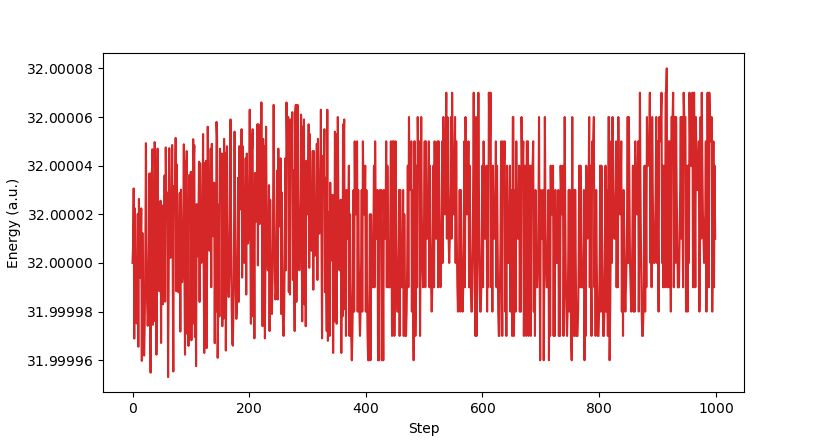
\includegraphics[width=\linewidth]{Figure_1.png}	
\caption{Energy of the system as function of time.}
\end{figure}
The average velocity is measured after some time from the start of the simulation to allow equilibration:
\begin{figure}[h!]
	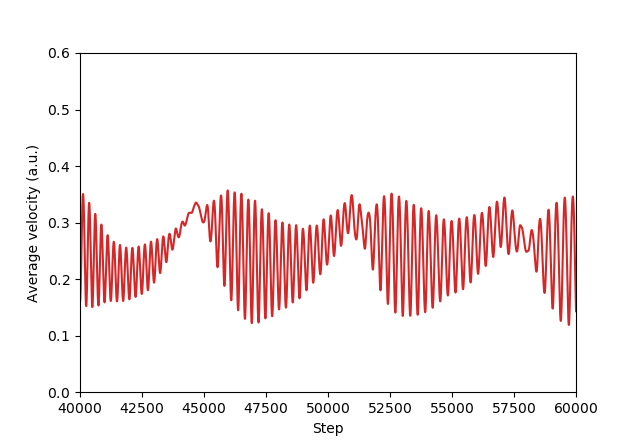
\includegraphics[width=\linewidth]{Figure_2.png}	
	\caption{Average velocity as a function of time. The total time of simulation is 1000 with a time step of 0.01 and 128 particles. }
\end{figure}

\section{Conclusions}

\end{document}